\documentclass{article}
\usepackage[utf8]{inputenc}
\usepackage[italian]{babel}
\usepackage{amsmath}
\usepackage{amssymb}
\usepackage{siunitx}
\usepackage{tabularray}
\usepackage{graphicx}
\usepackage{float}
\newcommand*{\best}[1]{{#1}_\text{best}}
\newcommand*{\errrel}[1]{\frac{\delta #1}{{#1}_\text{best}}}
\title{
    Laboratorio di Fisica 1\\
    R3: Misura del modulo del campo gravitazionale locale
}
\author{Gruppo 17: Bergamaschi Riccardo, Graiani Elia, Moglia Simone}
\date{18/10/2023 – 25/10/2023}
\makeindex
\begin{document}

\maketitle

\begin{abstract}
    Il gruppo di lavoro ha misurato indirettamente il modulo del campo gravitazionale locale con due metodi distinti:
    dapprima facendo cadere due palline da ferme, successivamente tenendo conto di distanze diverse e velocità iniziali diverse.
\end{abstract}

\section{Materiali e strumenti di misura utilizzati}
\begin{center}
    \begin{tblr}{ |Q[l,m]|Q[c,m]|Q[c,m]|Q[c,m]| }
        \hline
        \textbf{Strumento di misura} & \textbf{\:\:\:\:Soglia\:\:\:\:} & \textbf{Portata} & \textbf{Sensibilità} \\
        \hline
        {Fototraguardi con \\ contatore di impulsi} & \qty{1}{\micro s} & \qty{99999999}{\micro s} & \qty{1}{\micro s} \\
        \hline[dashed]
        Metro a nastro & \qty{0.1}{cm} & \qty{300.0}{cm} & \qty{0.1}{cm} \\
        \hline[dashed]
        Micrometro ad asta filettata & \qty{0.01}{mm} & \qty{25.00}{mm} & \qty{0.01}{mm} \\
        \hline
        \textbf{Altro} & \SetCell[c=3]{l} \textbf{Descrizione/Note} \\
        \hline
        Sistema di sgancio elettropneumatico & \SetCell[c=3]{l} {
            Usato, tramite comando manuale, per rilasciare \\
            le sferette in modo riproducibile.
        } \\
        \hline[dashed]
        {Due sferette \\ (con diametri distinti)} & \SetCell[c=3]{l} {
            Indicheremo con $A,B$ le due sferette; il diametro \\
            di $A$ è $\left(24.63\:\pm\:0.01\right)\unit{mm}$, mentre quello \\
            di $B$ è $\left(22.23\:\pm\:0.01\right)\unit{mm}$.
        } \\
        \hline[dashed]
        Livella & \SetCell[c=3]{l} {
            Utile per assicurarsi che i fototraguardi \\
            siano orizzontali.
        } \\
        \hline
    \end{tblr}
\end{center}

\section{Esperienza e procedimento di misura}
\subsection{Misurazione di $\vec{g}$ con $v_0=0$}
\begin{enumerate}
    \item Misuriamo con il metro a nastro la distanza $d_0$ tra il sistema di sgancio e il fototraguardo.
          Detto $\varnothing_i$ il diametro dell'$i$-esima pallina, la distanza percorsa dalla pallina
          nel tempo che misureremo sarà allora $d_0 - \frac{1}{2}\varnothing_i$.
    \item Dopo aver acceso e impostato il contatore di impulsi adeguatamente facciamo cadere la sferetta
          attraverso il sistema di sgancio, ottenendo così il suo tempo di caduta: eseguiamo questa misura
          100 volte per ognuna delle due sferette.
\end{enumerate}


Di seguito sono riportate le misure così ottenute:
\[d_0 = \left(125.9\pm 0.1\right)\unit{cm}\]

\begin{center}\begin{tblr}{ |c|c|c|c| }
    \hline
        {\textbf{Grave} \\ $i$} &
        {\textbf{Massa} \\ $m_i$ (\unit{g})} &
        {\textbf{Posizione} \\ $x_i$ (\unit{cm})} &
        {\textbf{Allungamento} \\ $\left(\Delta x\right)_i$ (\unit{cm})} \\
    \hline
    $A$     & $  407,73\:\pm\:0.01$ & $ 7,9\:\pm\:0.1$ & $ 4,6\:\pm\:0.2$ \\
    $B$     & $  542,47\:\pm\:0.01$ & $ 9,6\:\pm\:0.1$ & $ 6,3\:\pm\:0.2$ \\
    $C$     & $  667,82\:\pm\:0.01$ & $11,3\:\pm\:0.1$ & $ 8,0\:\pm\:0.2$ \\
    $A+B$   & $  950,22\:\pm\:0.01$ & $14,4\:\pm\:0.1$ & $11,1\:\pm\:0.2$ \\
    $A+C$   & $ 1085,56\:\pm\:0.01$ & $15,9\:\pm\:0.1$ & $12,6\:\pm\:0.2$ \\
    $B+C$   & $ 1220,28\:\pm\:0.01$ & $17,5\:\pm\:0.1$ & $14,2\:\pm\:0.2$ \\
    $A+B+C$ & $ 1628,02\:\pm\:0.01$ & $22,2\:\pm\:0.1$ & $18,9\:\pm\:0.2$ \\
    \hline
\end{tblr}\end{center}

Per determinare la costante elastica $k$ della molla, abbiamo effettuato
una regressione lineare (non pesata) dei dati così ottenuti, facendo
riferimento alla seguente relazione (che segue direttamente dalla legge
di Hooke, ponendo $F_\text{elastica}$ = $F_\text{peso}$):
\[\Delta x = \frac{g}{k} m\]
Detto $b=\best{b}\pm\delta b$ il coefficiente angolare della retta di regressione, vale allora:
\[k = \errrel{g} \qquad\wedge\qquad \errrel{k} = \errrel{g} + \errrel{b}\]
Si noti che l'intercetta della retta di regressione dev'essere compatibile con $0$.

\emph{
    \textbf{Osservazione}.
    $g$ non può essere considerata una costante nota con certezza,
    poiché, secondo la legge di gravitazione universale, $g$ dipende
    dalla distanza dal centro di massa della Terra: che $g$ sia costante
    al variare della posizione del grave è solo un'approssimazione.
    Pertanto, abbiamo considerato
    $g=\left(9.81\pm0.01\right)\unit{m\per s^2}$.
}

Ecco la retta di regressione e i relativi risultati:
\begin{figure}[H]
    %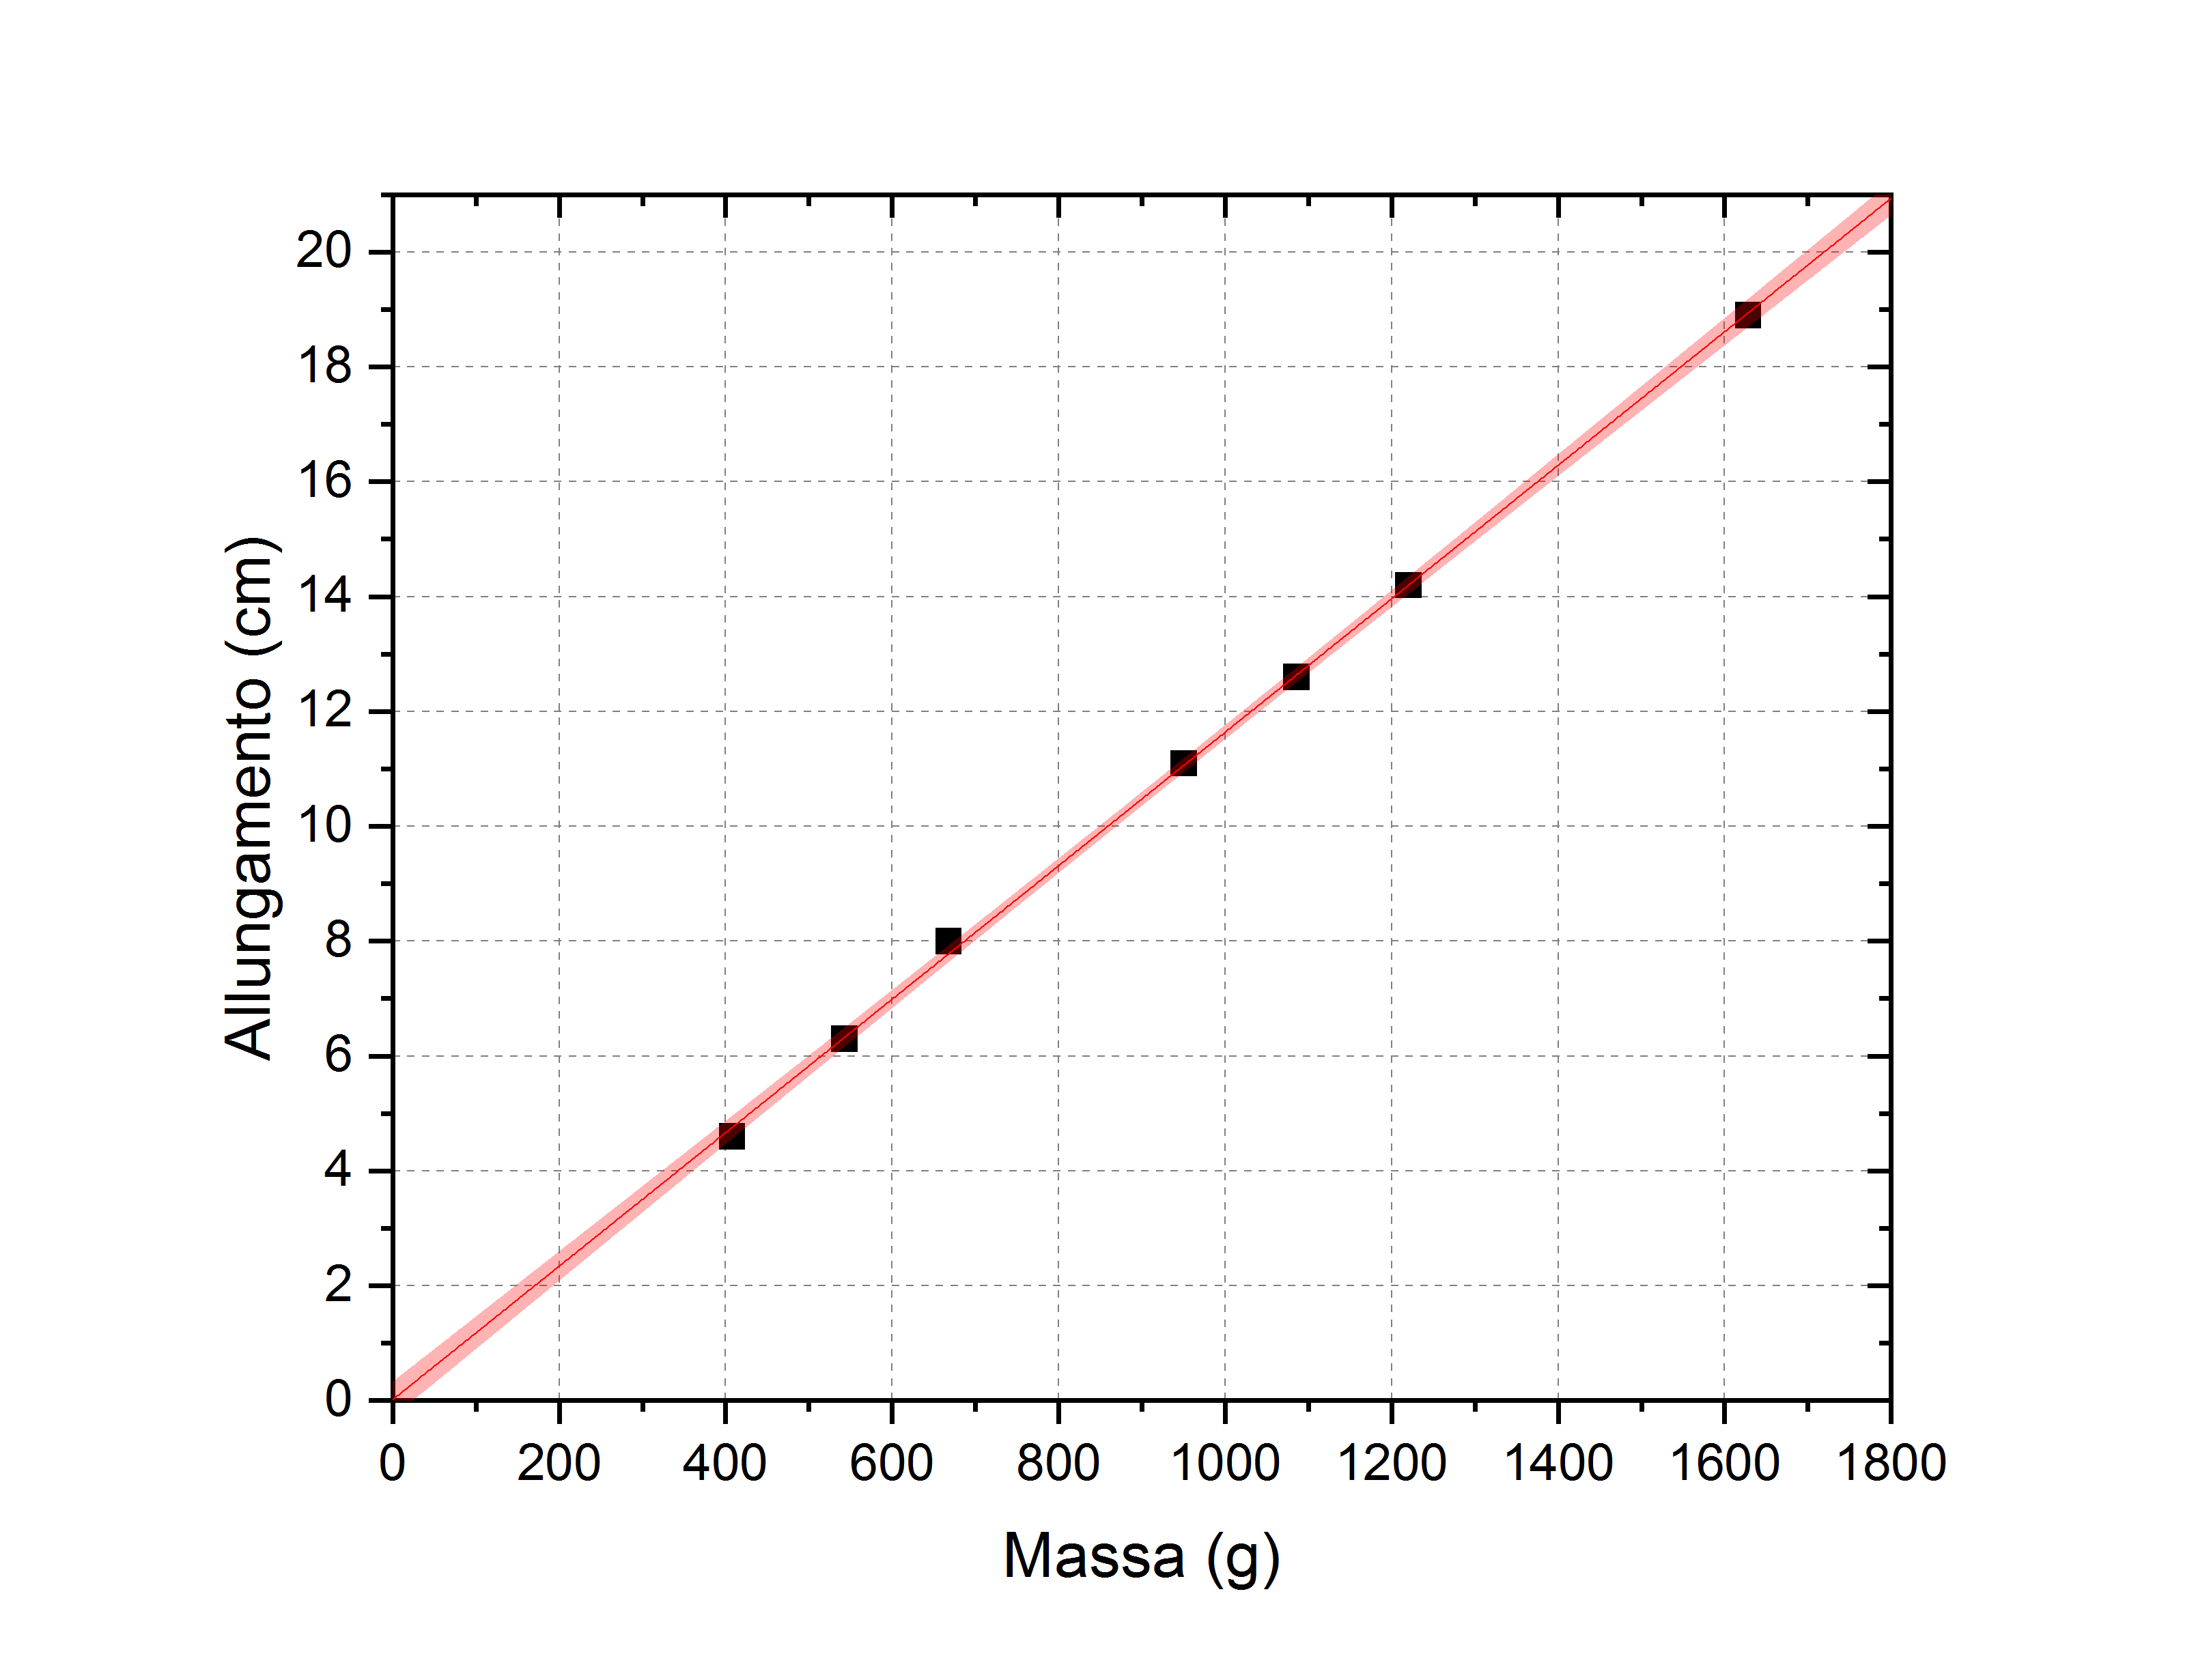
\includegraphics[trim={0 1.8cm 0 0},width=\textwidth]{SaticoReg.jpg}
    \caption{
        La retta di regressione (in rosso)
        e la sua regione di incertezza (in rosa).
    }
\end{figure}
\begin{itemize}
    \item $a = \left(0.02\pm0.12\right)\unit{cm}$ (compatibile con 0)
    \item $
        b = \left(11.62\pm0.12\right)\cdot10^{-3}\;\unit{cm\per g}
          = \left(11.62\pm0.12\right)\cdot10^{-2}\;\unit{m\per kg}
    $
    \item $k = \left(84.4\pm0.8\right)\unit{N\per m}$
\end{itemize}

\subsection{Misurazione del campo gravitazionale con $v_0\ne0$}
\begin{enumerate}
    \item Consideriamo la distanza tra i due fototraguardi e impostiamo i fotodiodi
          del contatore su A+B.
    \item Usando solo
    \begin{enumerate}
        \item Appeso il campione alla molla, allineiamo i due fototraguardi
              aiutandoci con la livella, in modo tale che possano rilevare
              le oscillazioni nel modo più accurato possibile;
        \item Tiriamo leggermente il campione verso il basso e poi lo rilasciamo,
              in modo che il sistema molla inizi a oscillare con direzione
              il più possibile parallela a $\vec{g}$;
        \item Attesa la stabilizzazione dell’oscillazione, avviamo
              l'acquisizione della misura di un tempo (20 periodi)
              $20T_i$.
        \item Ripetiamo molte volte (in tutto $N_{20T_i}$) i punti
              (b) e (c). In particolare, $N_{20T_A} = N_{20T_B} = 25$
              e $N_{20T_C} = N_{20T_{A+B}} = 30$.
    \end{enumerate}
    \item Infine, misuriamo con la bilancia, separatamente,
          la massa della molla $m_m$ e la massa del gancio $m_g$.
\end{enumerate}

Infatti, nel caso dinamico, il contributo di queste masse
\emph{non} si annulla; in particolare, la massa del gancio
contribuisce appieno (in quanto è solidale col grave),
mentre la massa della molla contribuisce per circa
$\frac{1}{3}$. La massa effettiva da considerare per ogni grave
sarà allora:
\[\best{\left(\left(m_\text{eff}\right)_i\right)} = \best{\left(m_i\right)} + \best{\left(m_g\right)} + \frac{1}{3}\best{\left(m_m\right)}\]
\[\delta \left(m_\text{eff}\right)_i = \delta m_i + \delta m_g + \frac{1}{3}\delta m_m\]

Di seguito sono riportate le distribuzioni dei dati raccolti:

\begin{figure}[H]
    %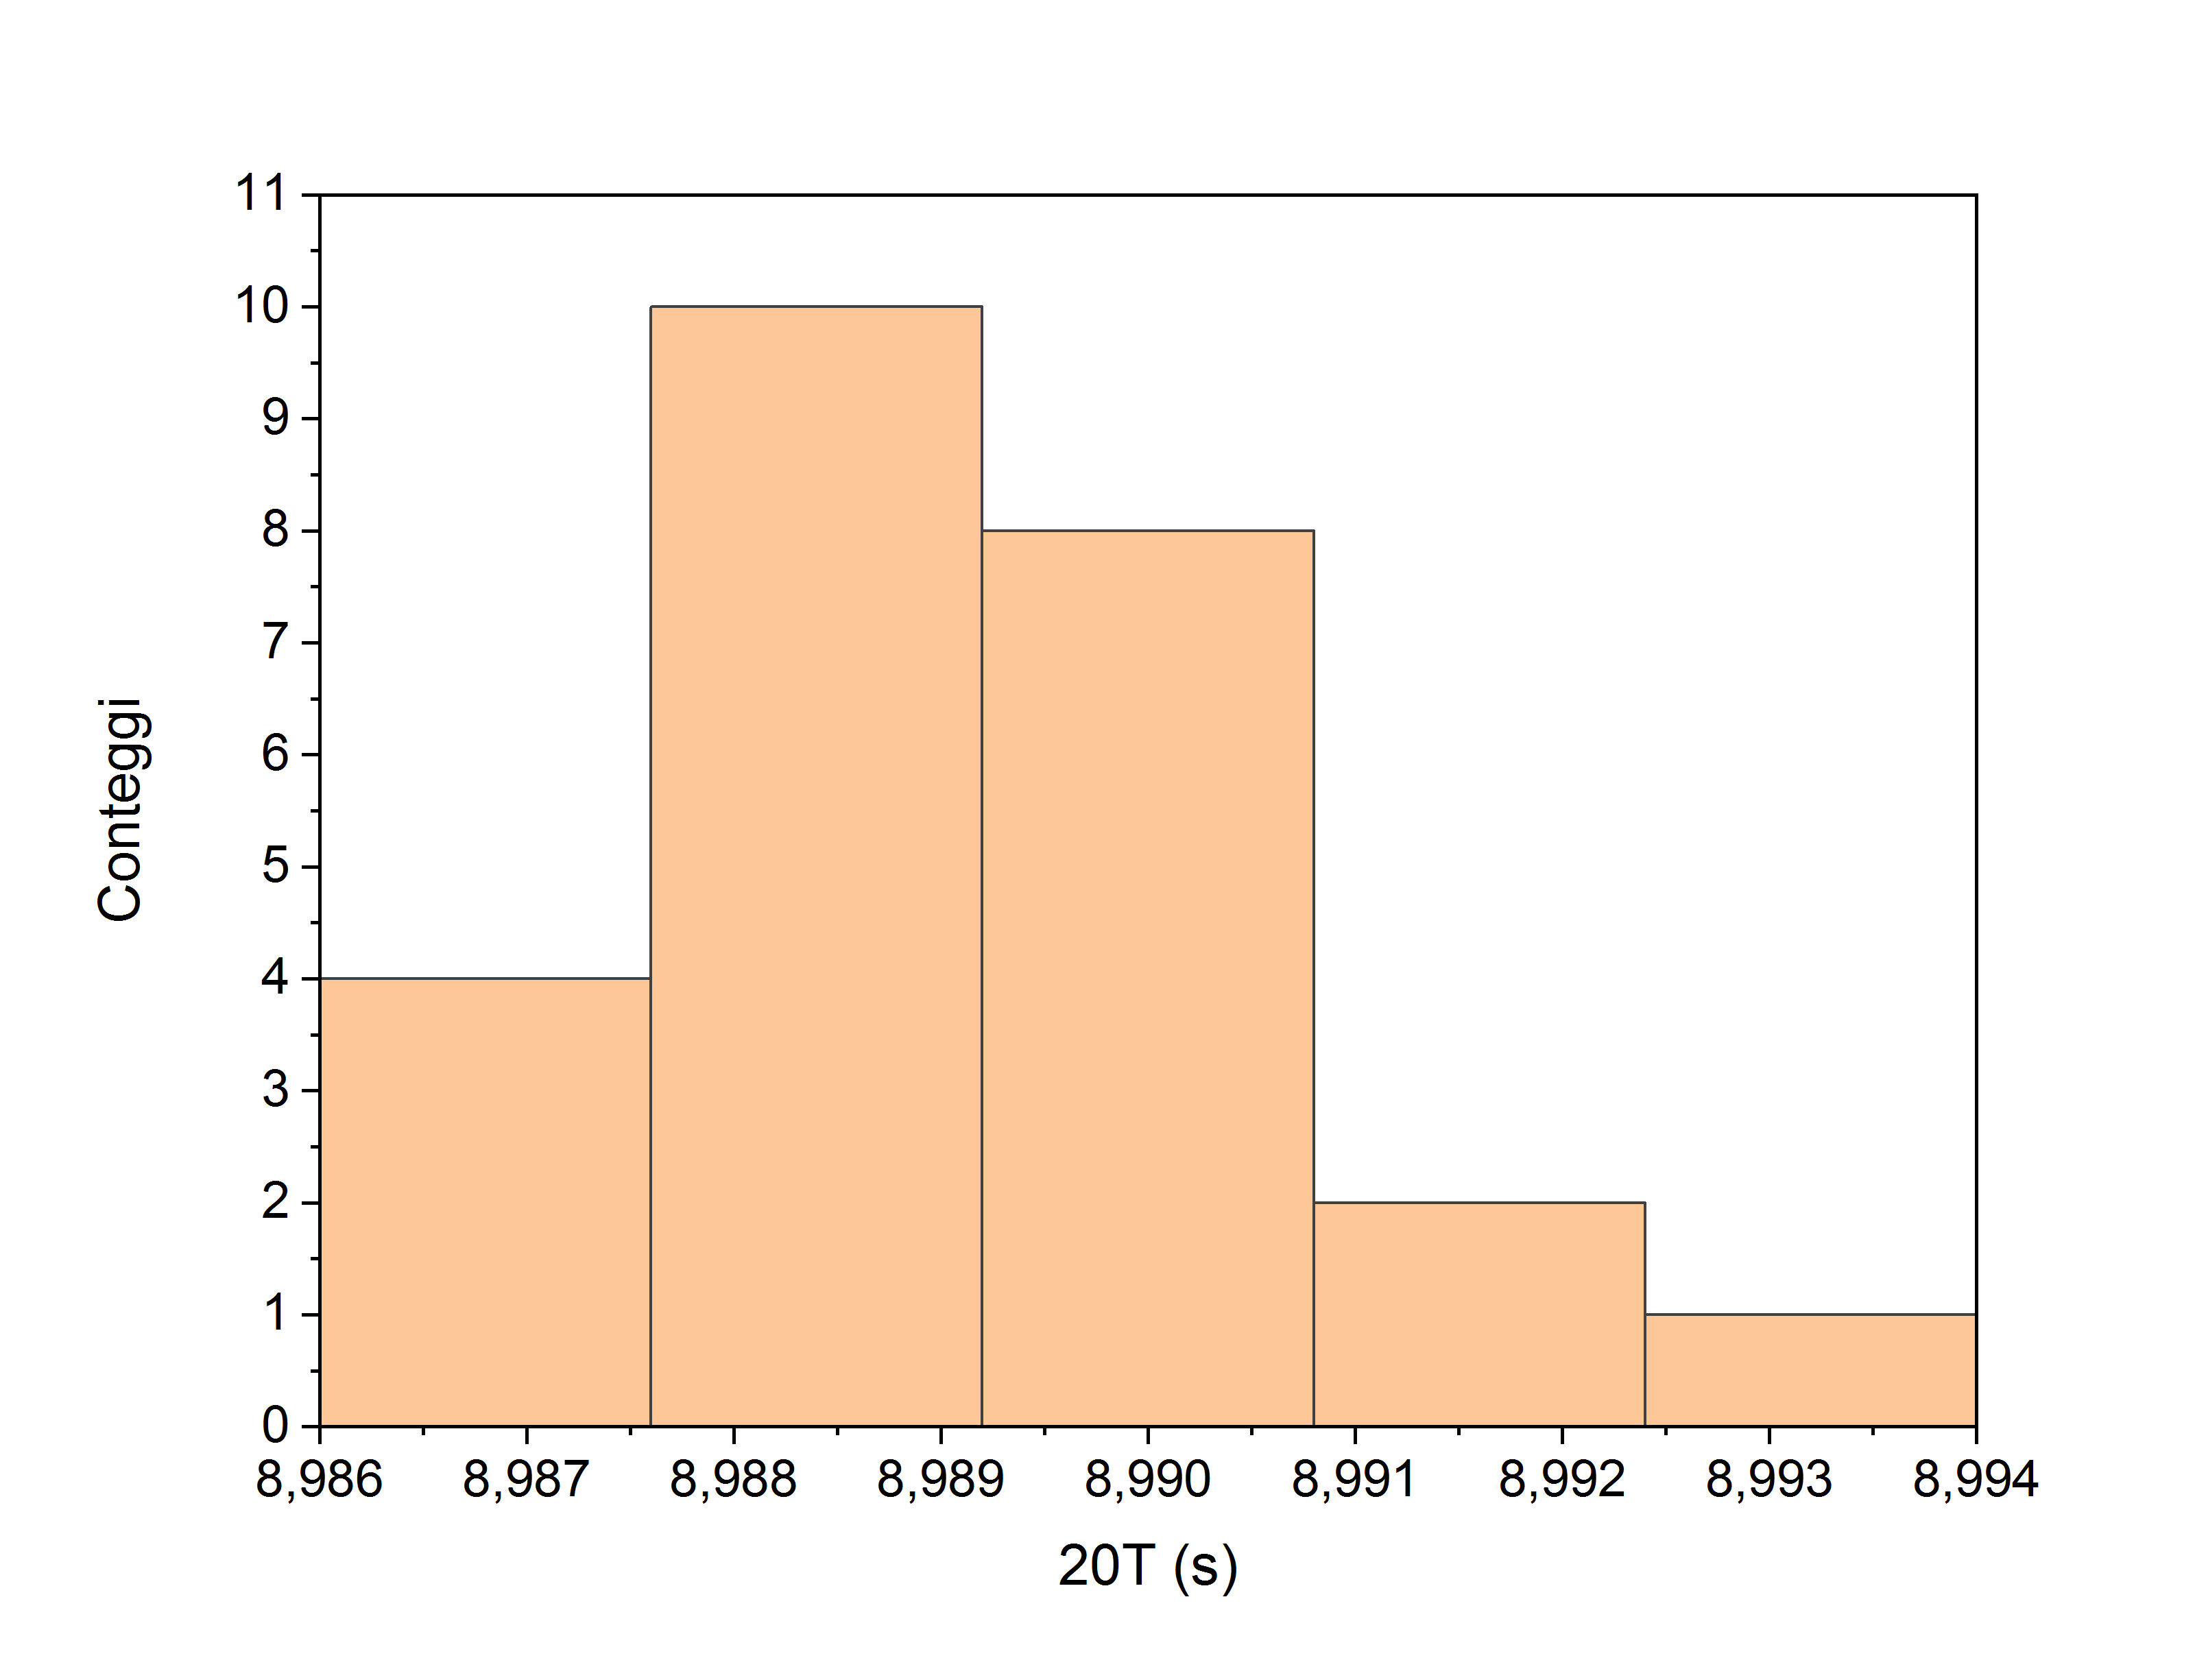
\includegraphics[trim={2cm 1.8cm .7cm 1.5cm},width=.5\textwidth]{Dinamico1.jpg}
    %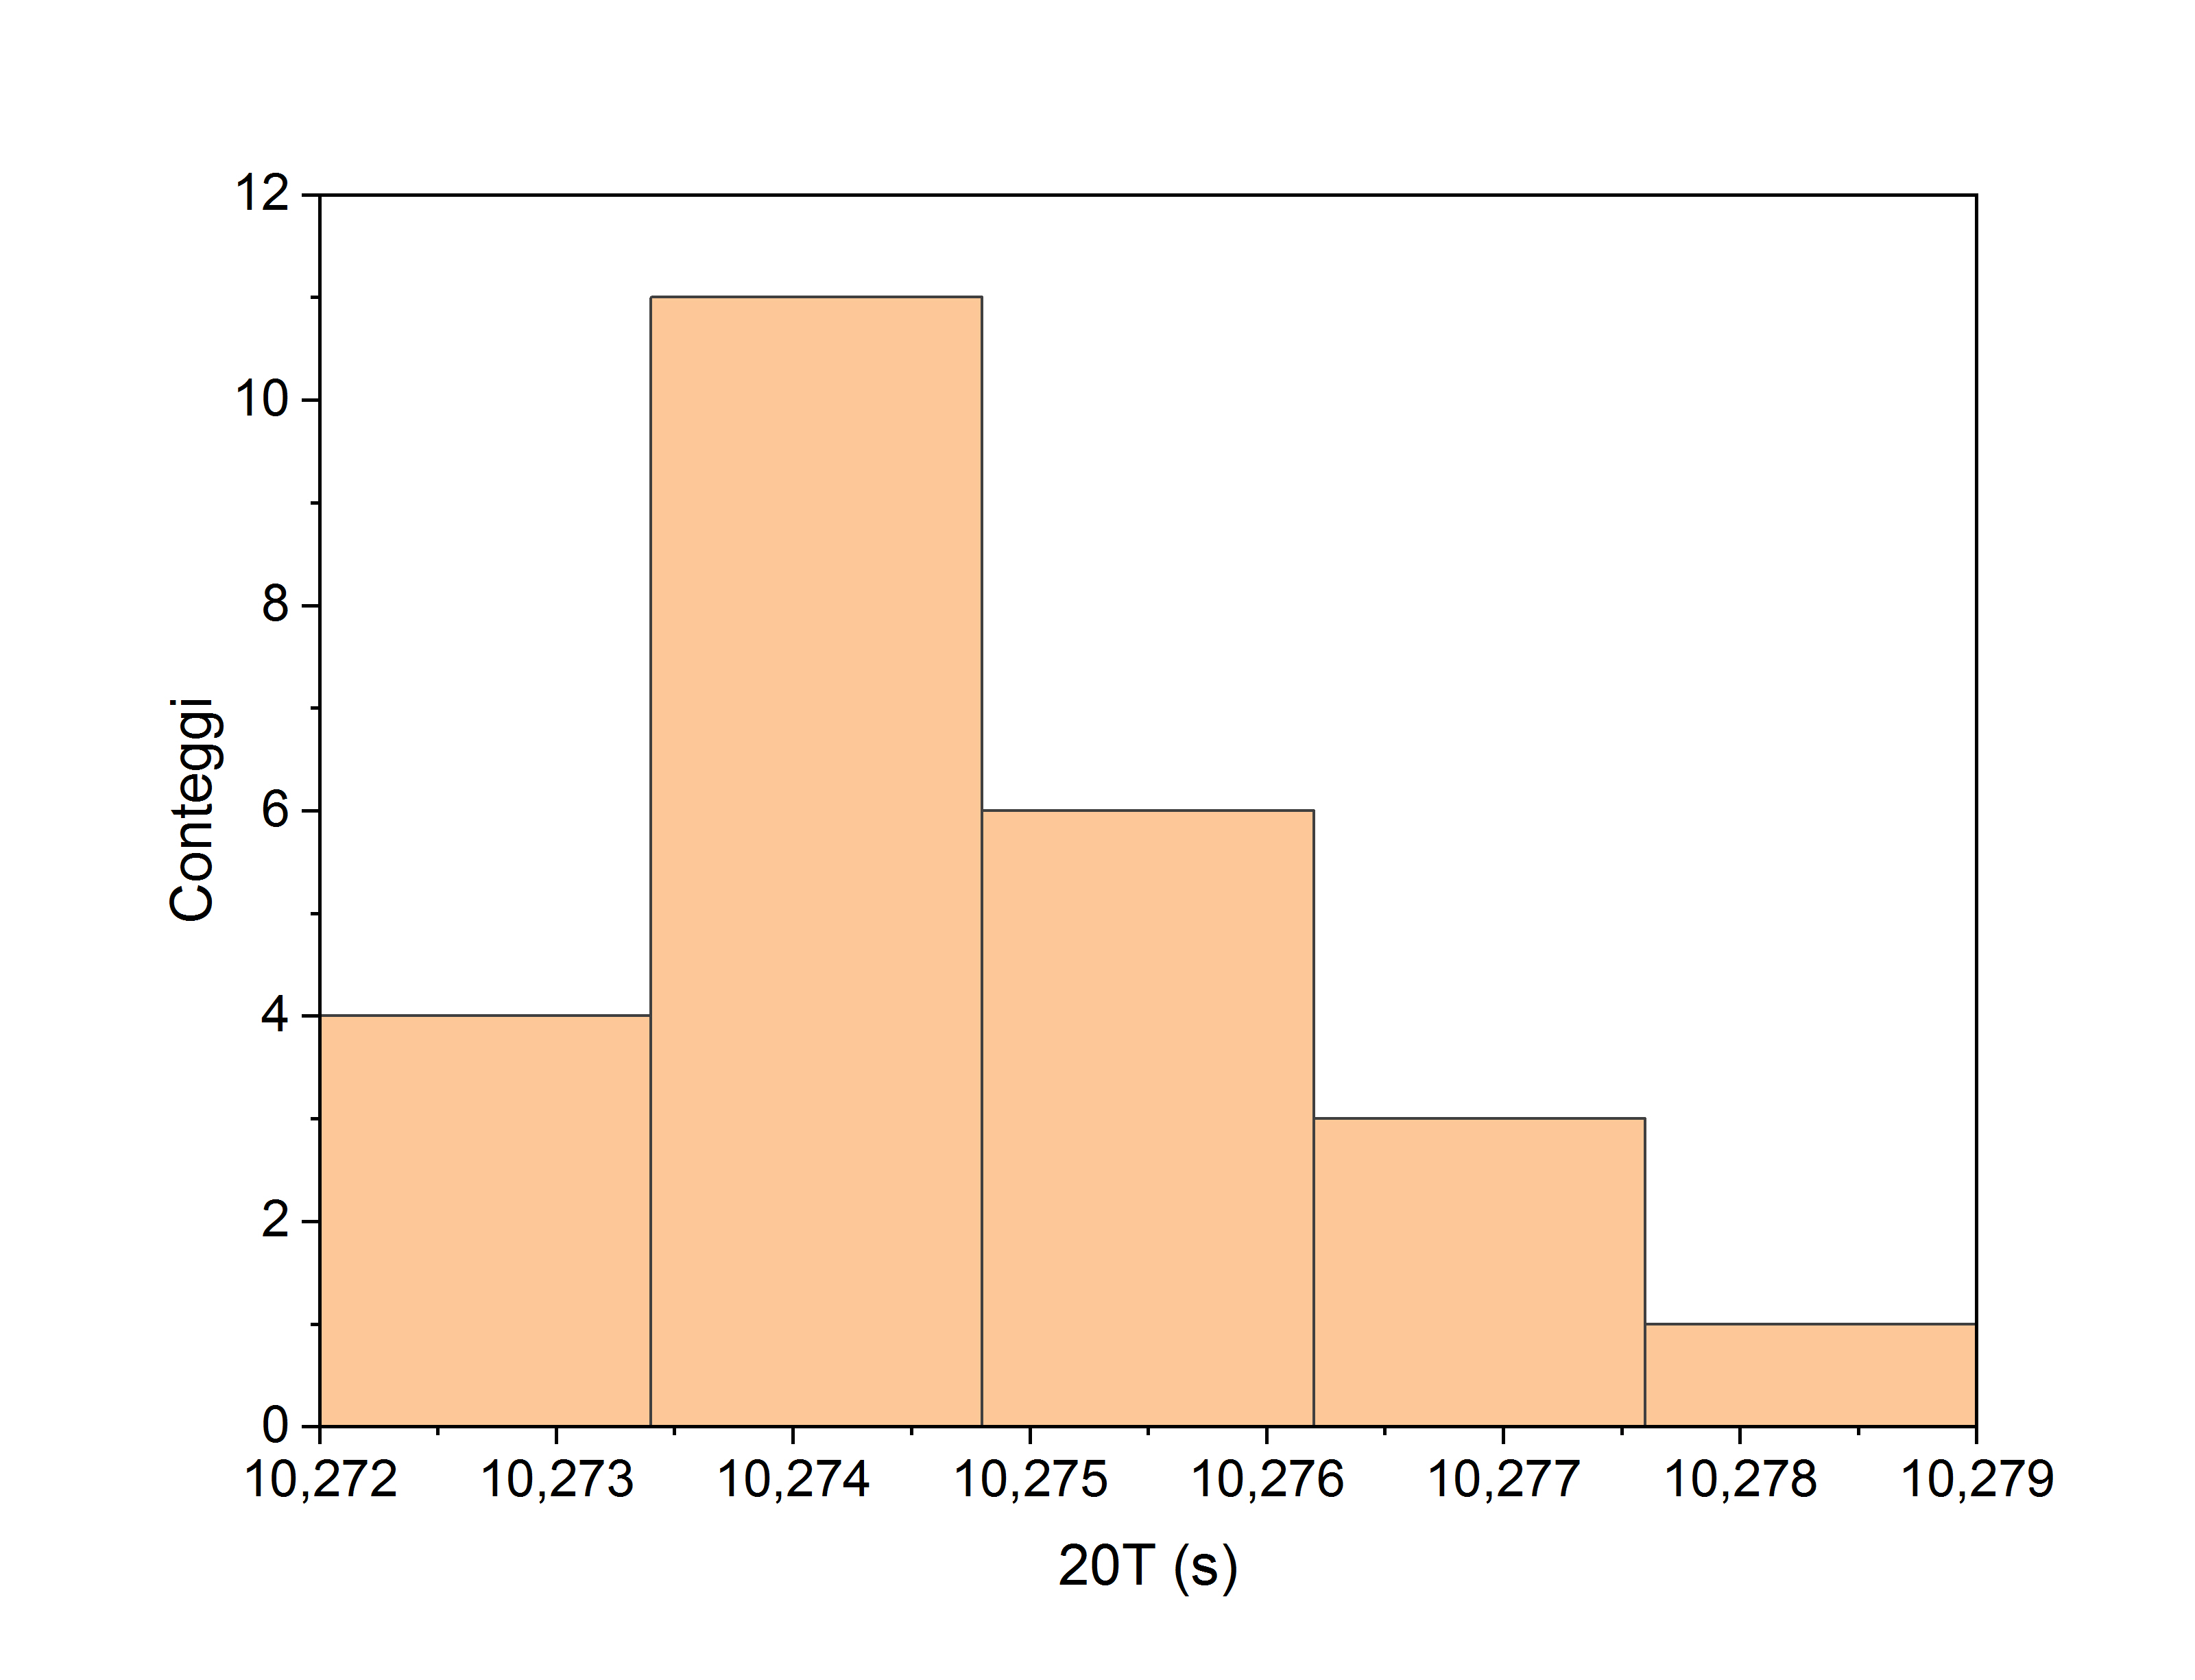
\includegraphics[trim={.7cm 1.8cm 2cm 1.5cm},width=.5\textwidth]{Dinamico2.jpg}
    \caption{Istogrammi dei periodi delle oscillazioni di $A$ e $B$}
\end{figure}\begin{figure}[H]
    %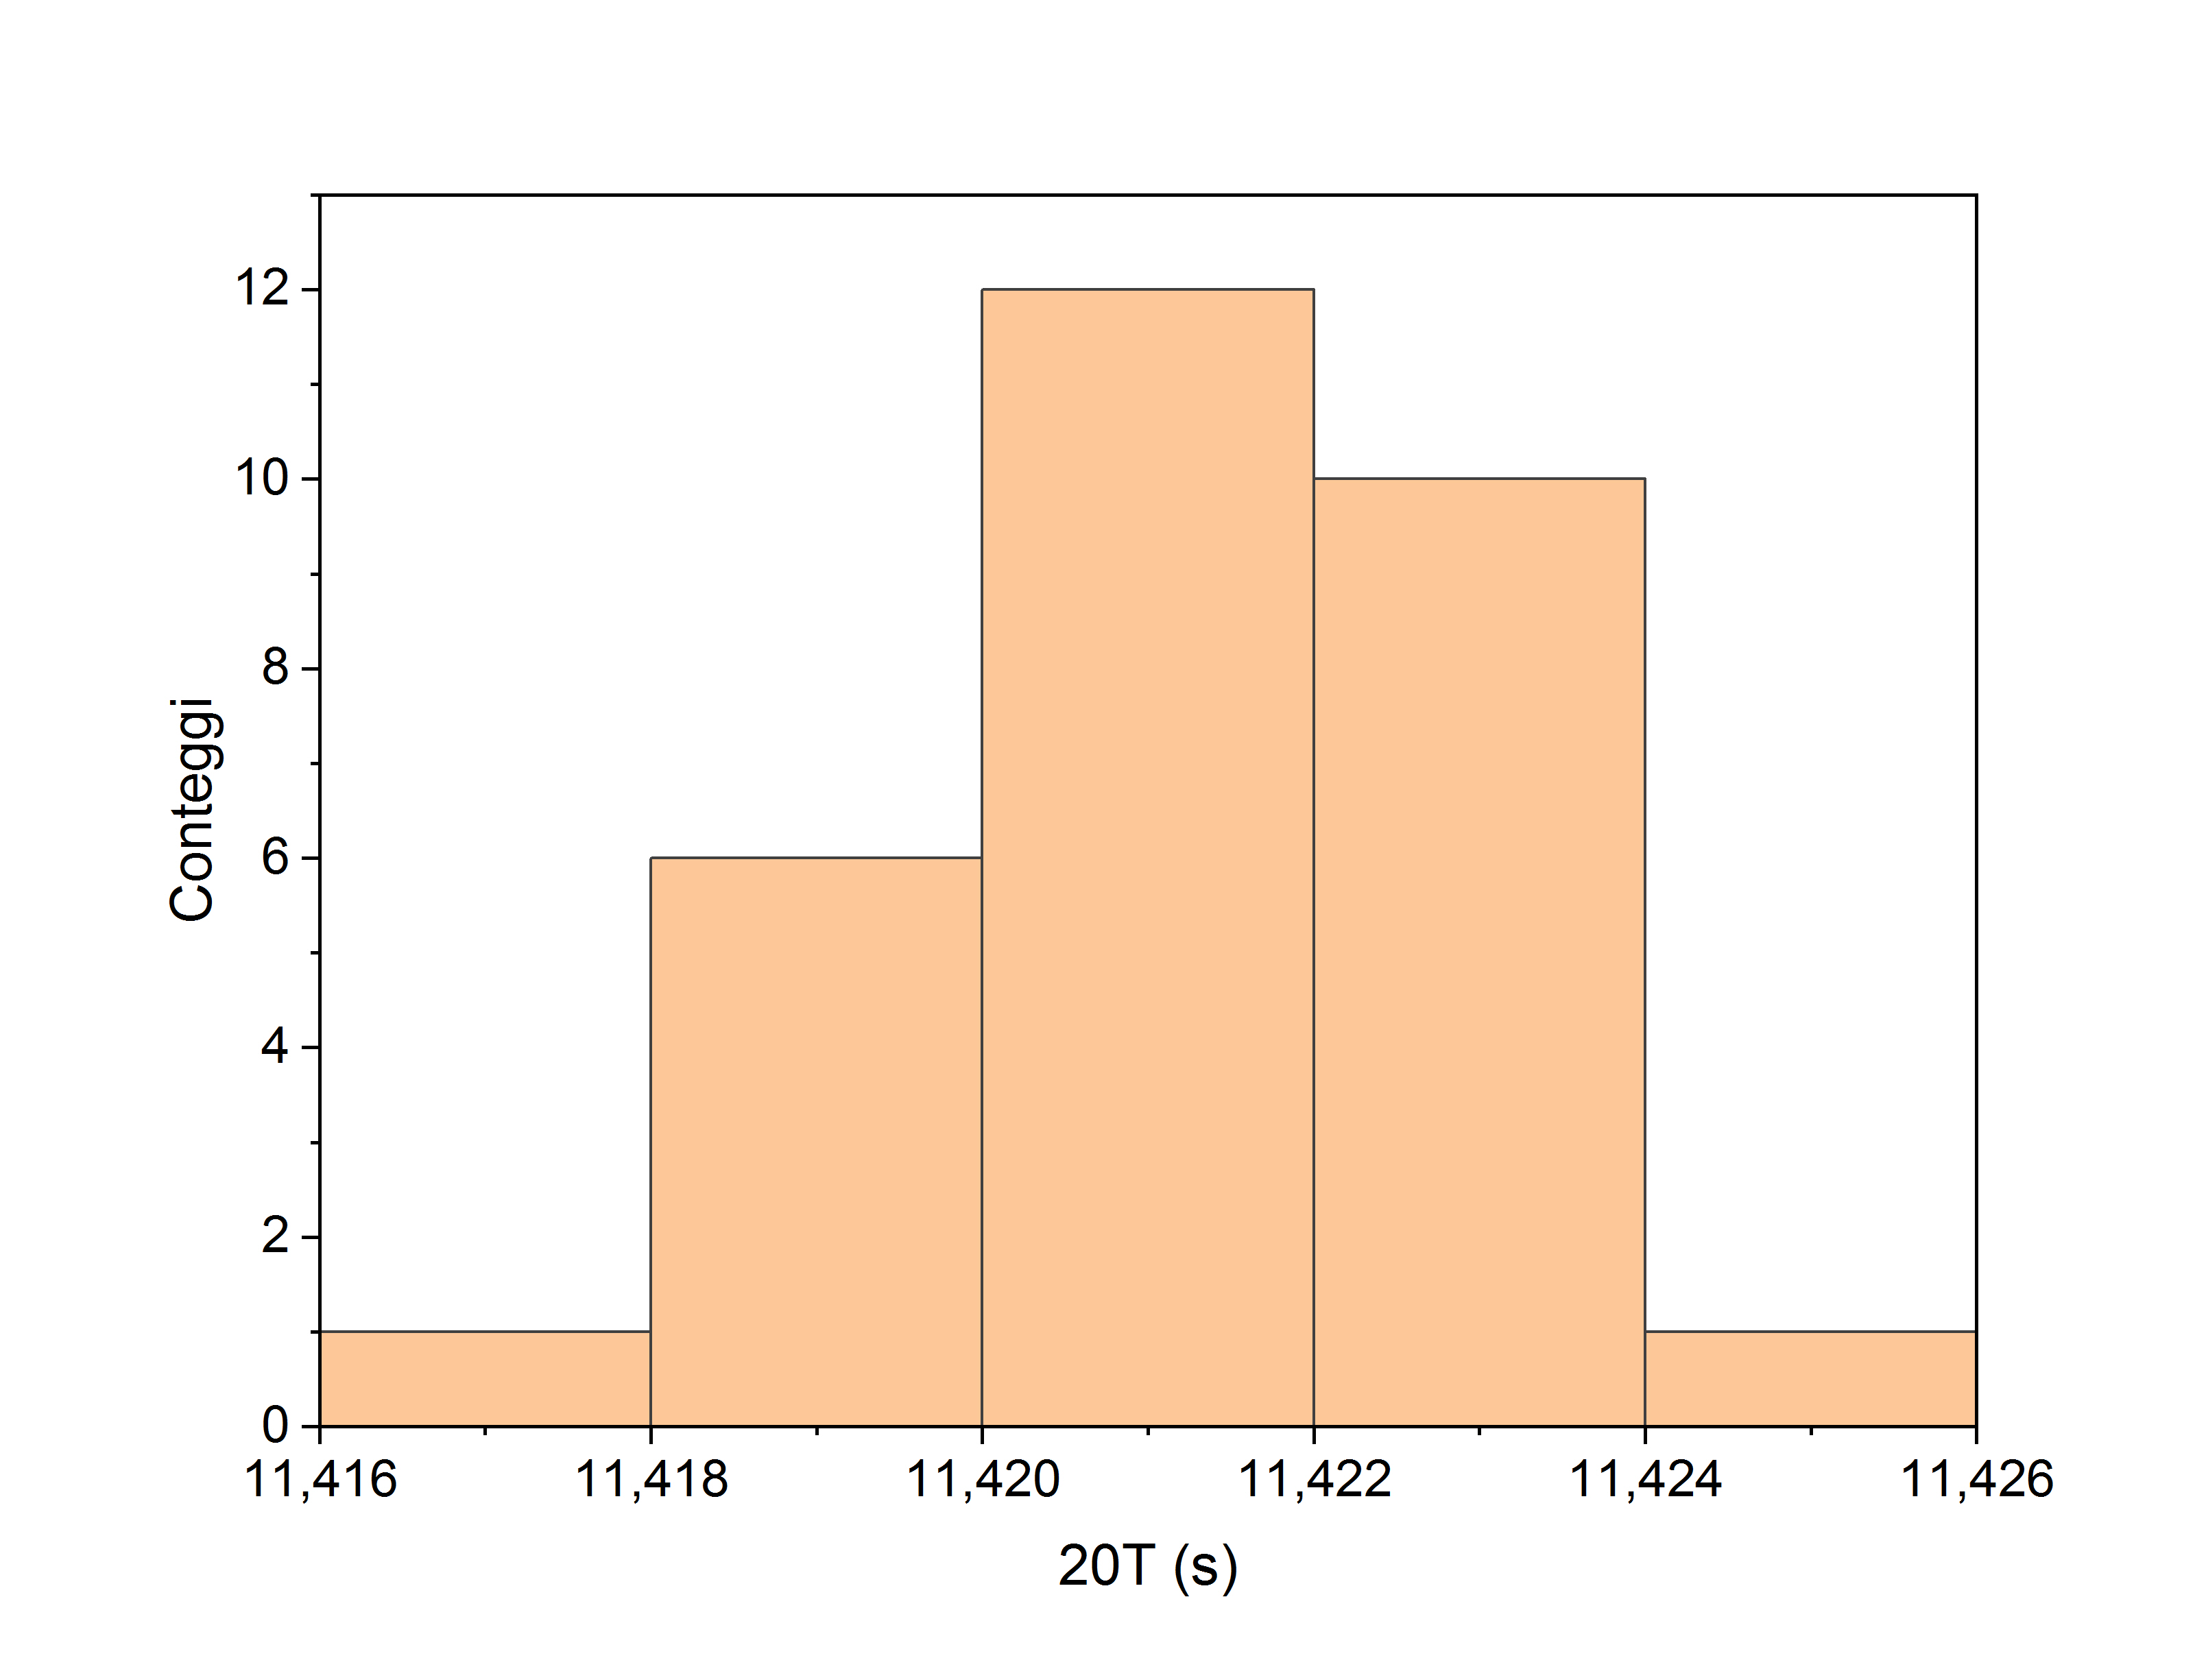
\includegraphics[trim={2cm 1.8cm .7cm 1.5cm},width=.5\textwidth]{Dinamico3.jpg}
    %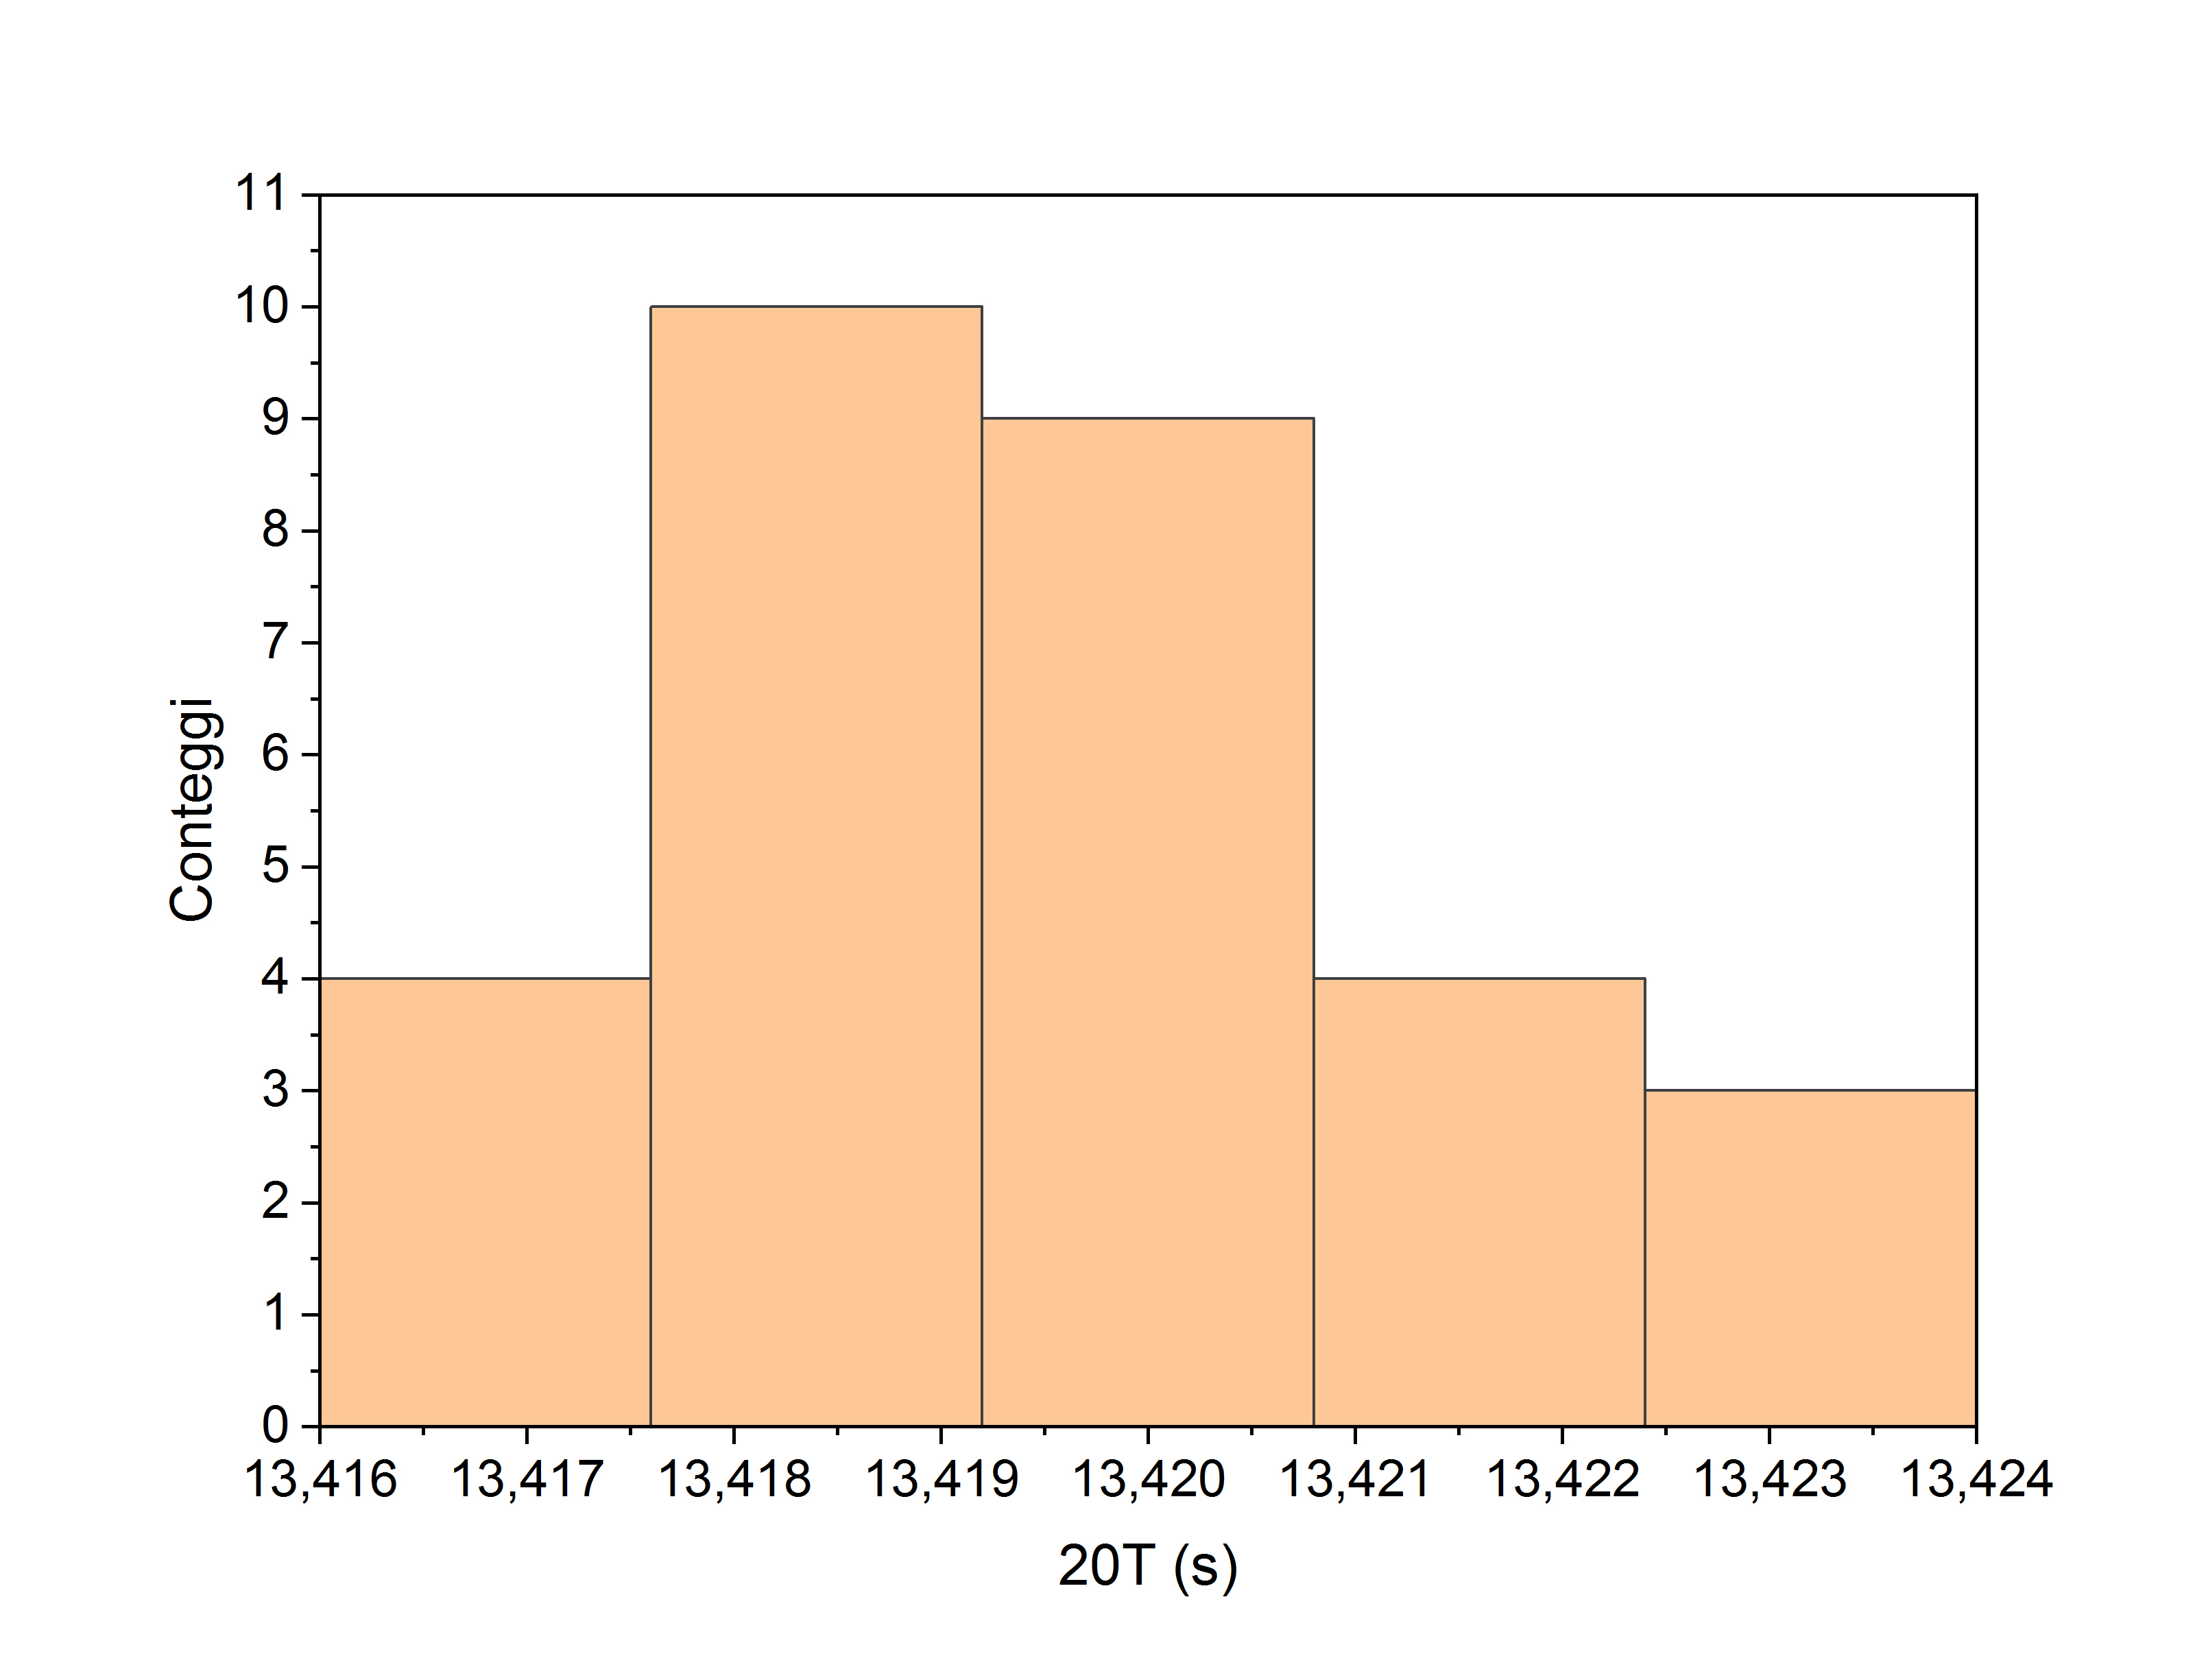
\includegraphics[trim={.7cm 1.8cm 2cm 1.5cm},width=.5\textwidth]{Dinamico4.jpg}
    \caption{Istogrammi dei periodi delle oscillazioni di $C$ e $A+B$}
\end{figure}

Poiché i nostri dati hanno assunto distribuzioni grossolanamente
approssimabili a gaussiane, possiamo procedere al calcolo di $k$,
utilizzando, per ogni grave $i$, i seguenti valori:
\[
    \left(20T_i\right)_\text{best} = \overline{20T_i}
    \qquad\wedge\qquad
    \delta\left(20T_i\right) =
    \sigma_{\overline{20T_i}} =
    \frac{\sigma_{20T_i}}{\sqrt{N_{20T_i}}}
\]
dove $\overline{20T_i}$ e $\sigma_{20T_i}$ indicano rispettivamente
media e deviazione standard dei tempi.

Per determinare la costante elastica della molla, abbiamo effettuato
una regressione lineare (stavolta pesata) sui quadrati dei valori medi
dei tempi ($T_i^2$, con
$\delta T_i^2 = 5 \cdot 10^{-3} (20 T_i)_\text{best} \delta(20 T_i)$
)\footnote[2]{
    La formula per l'errore su $T_i^2$ segue direttamente dalla
    propagazione degli errori:
    \[
        \frac{\delta T_i^2}{\left(T_i^2\right)_\text{best}} = 2\frac{\delta T_i}{{\left(T_i\right)}_\text{best}}
        \qquad
        \delta T_i^2 = 2\left(T_i\right)_\text{best}\delta T_i
        \qquad
        \delta T_i^2 = \frac{\left(20T_i\right)_\text{best}(\delta 20T_i)}{200}
    \]
    da cui quanto riportato sopra.
    Si osservi che $\delta T_i^2$ dipende da
    $\left(20T_i\right)_\text{best}$:
    proprio questo è il motivo dietro alla scelta del metodo pesato
    per la regressione lineare.
} rispetto alla massa $\left(m_\text{eff}\right)_i$, facendo riferimento
alla relazione $T_i^2 = \frac{4\pi^2}{k} \left(m_\text{eff}\right)_i$. Allora, detto $b$ il
coefficiente angolare della retta di regressione, varrà:
\[
    k_\text{best}=\frac{4\pi^2}{b_\text{best}}
    \qquad\wedge\qquad
    \frac{\delta k}{k_\text{best}}=\frac{\delta b}{b_\text{best}}
\]
Si noti che, anche in questo caso, l'intercetta $a$ della retta dev'essere
compatibile con $0$.

Di seguito è riportata la retta di regressione, assieme ai risultati ottenuti:

\begin{figure}[H]
    %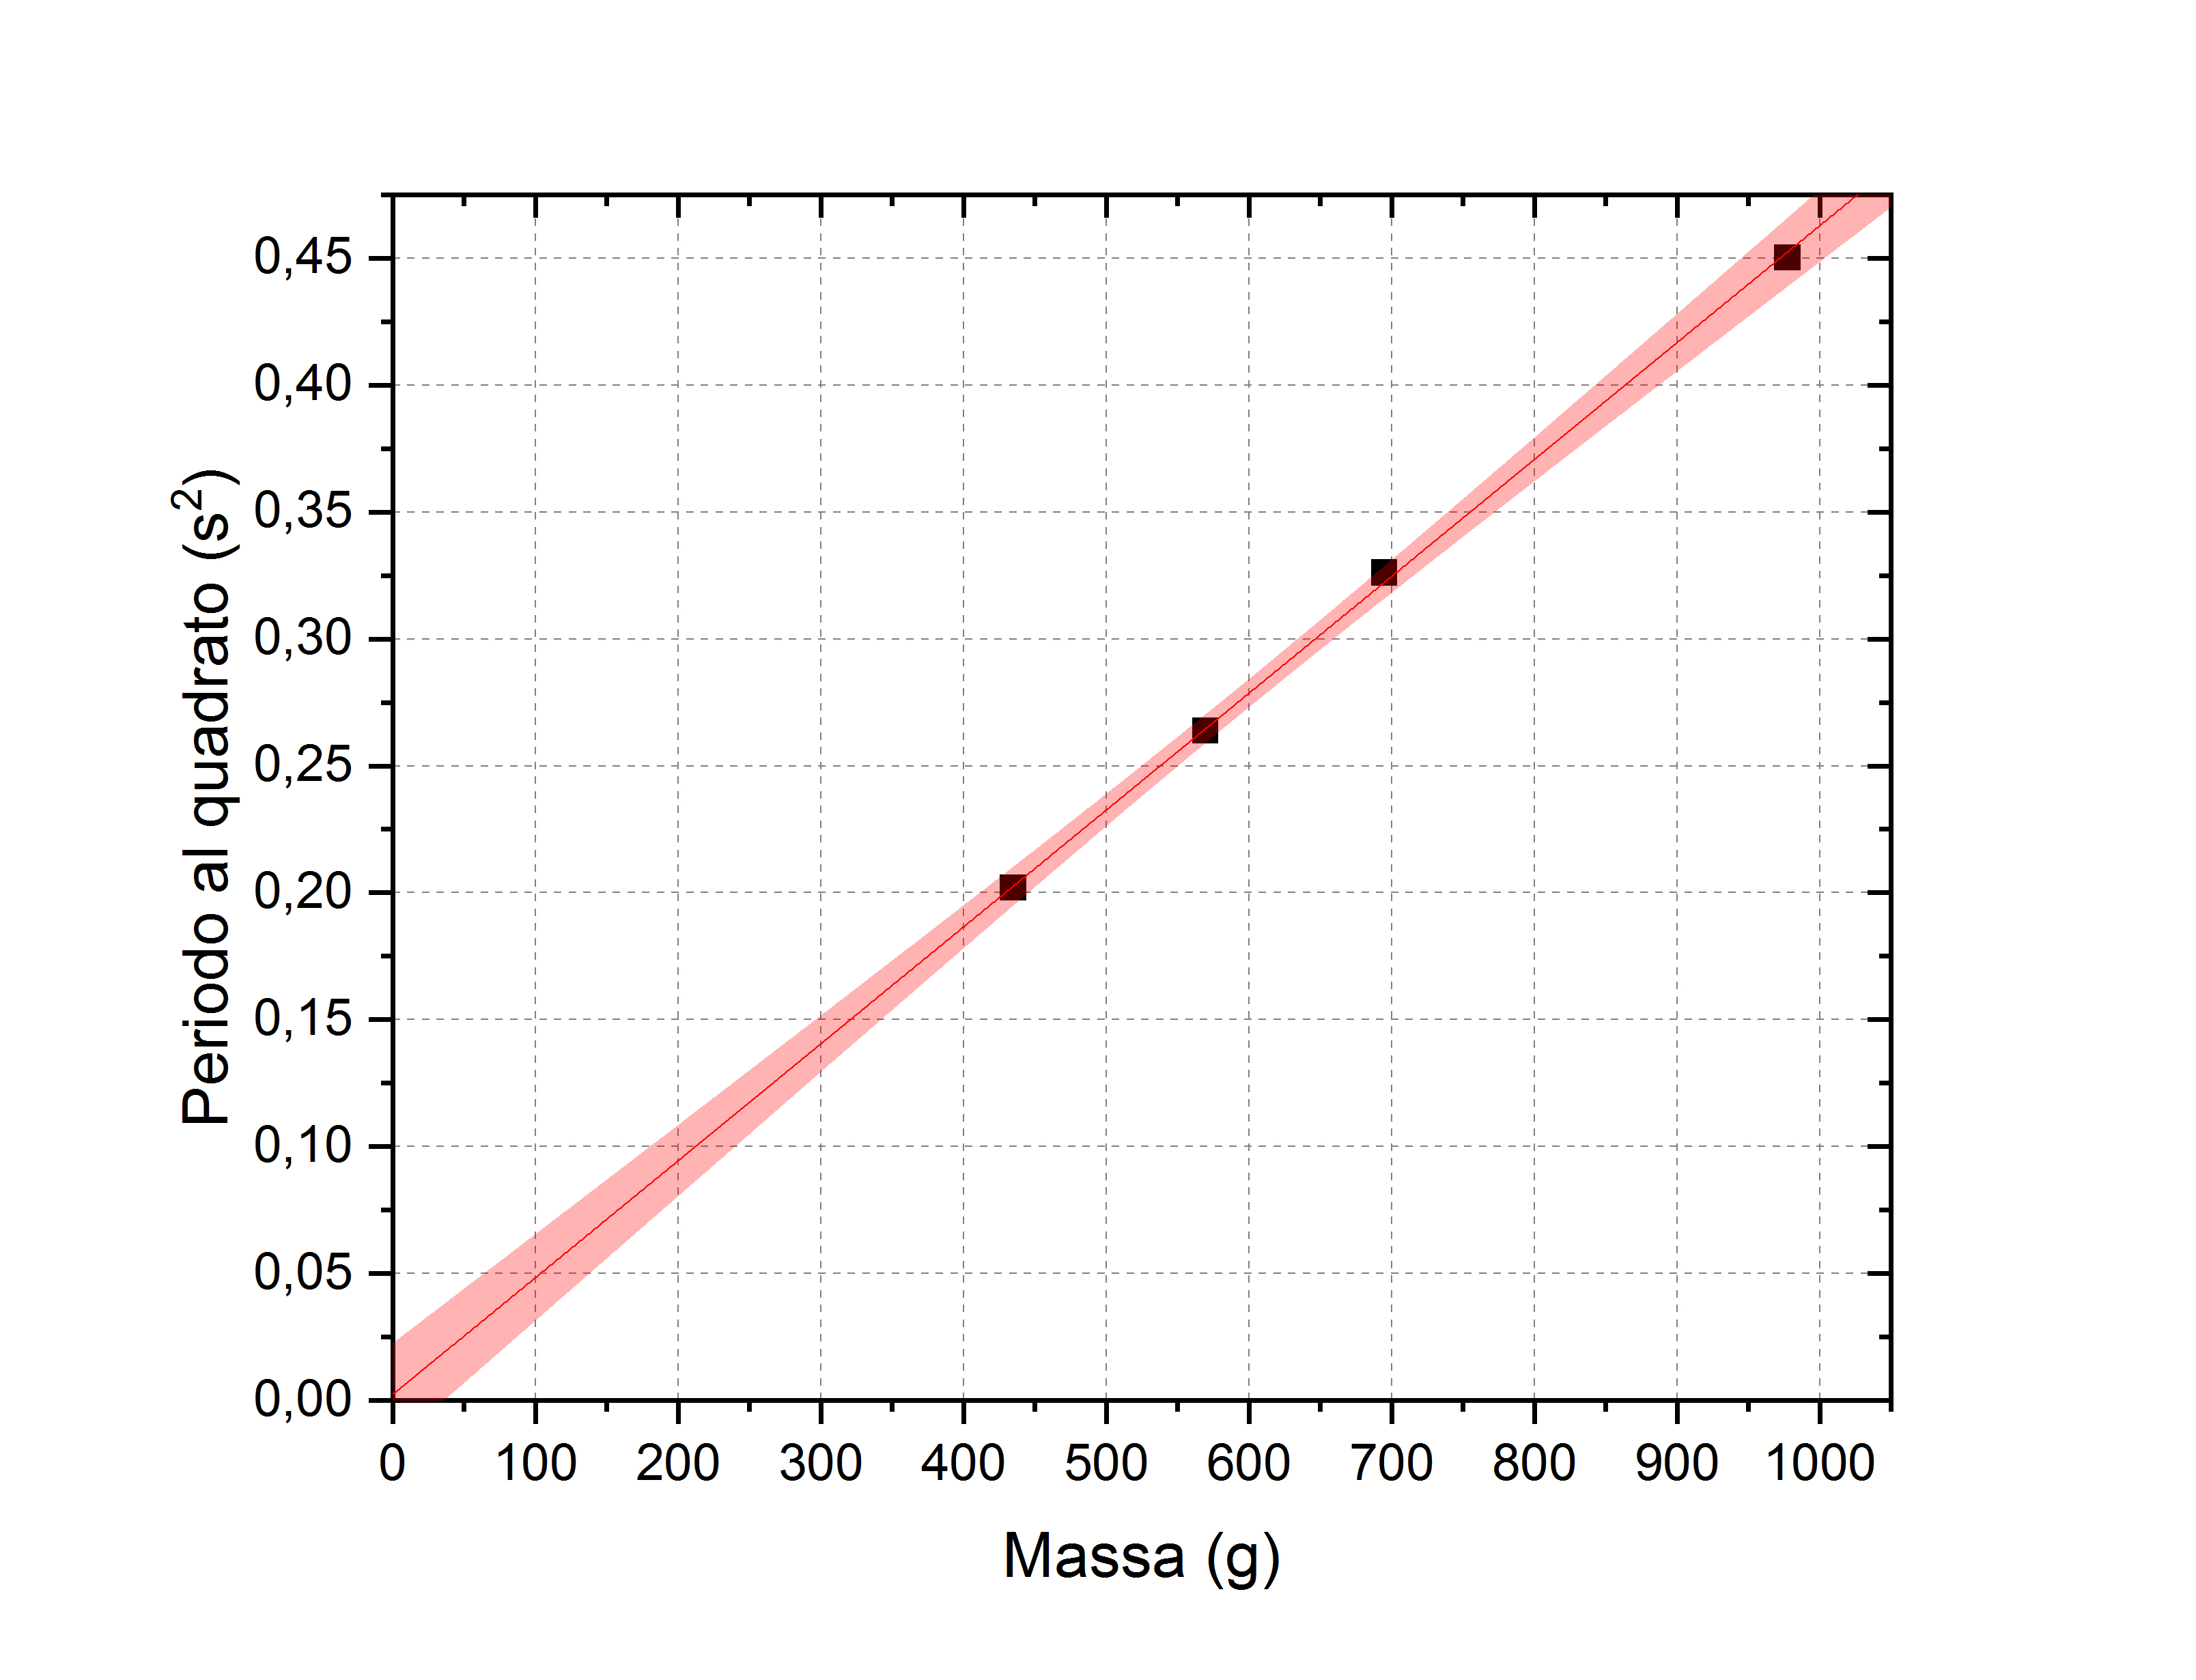
\includegraphics[trim={0 1.8cm 0 0},width=\textwidth]{DinamicoReg.jpg}
    \caption{
        La retta di regressione (in rosso)
        e la sua regione di incertezza (in rosa).
    }
\end{figure}

\begin{itemize}
    \item $a = \left(0.02\pm0.19\right)\unit{cm}$ (compatibile con 0)
    \item $
        b = \left(4.604\pm0.002\right)\cdot10^{-4}\;\unit{s^2\per g}
          = \left(46.04\pm0.02\right)\cdot10^{-2}\;\unit{s^2\per kg}
    $
    \item $k = \left(85.74\pm0.04\right)\unit{N\per m}$
\end{itemize}


\section{Conclusioni}
Per valutare numericamente la consistenza tra i due valori di $k$ ottenuti,
abbiamo calcolato il seguente valore (numero puro):
\[
    \varepsilon =
    \frac{
        \left|\left(k_\text{statica}\right)_\text{best} - \left(k_\text{dinamica}\right)_\text{best}\right|
    }{
        \delta k_\text{statica} + \delta k_\text{dinamica}
    }
\]
Allora $k_\text{statica}$ e $k_\text{dinamica}$ sono consistenti se e solo se $\varepsilon \le 1$.

Nel nostro caso, $\varepsilon = 1.33$. Il gruppo di lavoro ha ipotizzato che
questa inconsistenza (comunque contenuta, seppur non trascurabile) fra le due
misure possa essere ragionevolmente giustificata dalla difficoltà incontrata
nel ridurre al minimo le oscillazioni in direzione perpendicolare a $\vec{g}$;
considerato inoltre che la posizione dei fototraguardi non era ottimale, ciò
potrebbe avere ulteriormente influenzato la distribuzione dei tempi. È in
effetti possibile osservare che le distribuzioni da noi ottenute non sono,
il più delle volte, del tutto simmetriche: la moda sembra essersi spostata
leggermente a sinistra – un possibile sintomo dell'influenza di un
errore sistematico sulle misure.

\end{document}
